\chapter{Introduction}

\lettrine{A}{typical} configuration for high performance machines are clusters.
It means a team of individual processors or multiprocessors 
(and lately more specific 
hardware like GPUs) working together, interconnected by a super-fast network. 
The fundamental idea behind these big machines is getting speedup by mean of
partitioning the problem and parallelize the execution. So all processors (or a 
subset) inthe cluster will be dealing with different parts of the same problem 
and communicating between them in order to end up with a solution. For example 
imagine we have a weather forecast software, in order to speedup the forecast 
we can partition the surface of the earth and hold every portion to one individual
processor. The communication will be needed because the weather will also depend 
on surroundings, so every partition will need also information of other partitions 
results.

In Computer Science the discipline in charge to drive research in this field is 
the High Performance Computing, i.e. HPC. HPC has been increasing in importance 
and nowadays can be said it is the third support of science with theory and 
mathematics. The science that can be done thanks to this big machines goes from 
earthquake predictions to the analysis of the DNA of a carcinogenic cell, from
weather forecast to material physics simulation. HPC research is not just limited
to the hardware layer but drive research in all layers in the Transformation 
Hierarchy\cite{transformationHierarchy} in figure \ref{transformationHierarchyImg}.

\begin{figure}
  \caption{Levels of transformation}
  \label{transformationHierarchyImg}
  \centering
    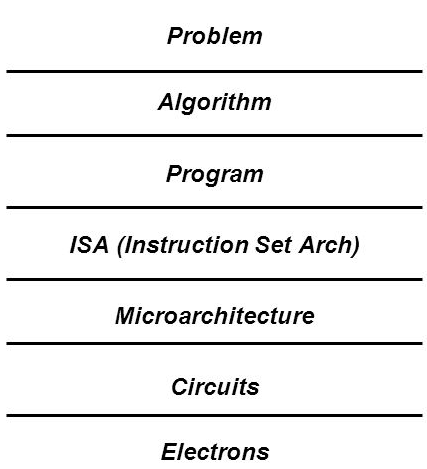
\includegraphics[width=100px]{transformationhierarchy.png}
\end{figure}

Resources are limited and expensive, so we have to be smart and use them in an
efficient way. Improving the efficiency is not just a matter that affects to one
layer of the stack but can be applied to every one of them. For example the
tremendous evolution of the last fourty years were improvements done mostly on
circuits layer what have been following the Moore's law \cite{moore:1965}. The
manufacturers have been reducing the size of transistors by a ration of 2 every
18 months as were predicted in figure \ref{moore-prediction}. Performance improvements 
were also at microarchitecture level with
disruptive designs that allows ILP like HPS\footnote{High Performance Substrace,
what is indeed out-of-order execution with in-order retirement.}
\cite{Patt:1985:HNM:18927.18916}, speculative execution with prefetchers, 
branch prediction or even memory access value speculation,
VLIW\footnote{Very Long Instruction Word} or TLP\footnote{Thread Level
Parallelism} with multi-threading. Improvements on memory hierarchy like cache 
associativitym, non-blocking cache or trace cache. The last
big revolution affected both architecture and program layers and was the 
multicore revolution. Was specially important because until then, programmers were 
agnostics, just feel their programs went faster but now, programs have to be 
architecture aware. With this last revolution a new effort for hide machine stuff
from programmers arise and end up with programming models like OpenMP
\cite{openmp_new}, OpenACC\cite{openacc_new} or OmpSs\cite{ompss_new}. A relatively
recent example is shown is this paper \cite{Alvarez:2015:CPT:2872887.2750411}
where they are trying to automatically use the fast scraptchpad memories by
means of compilers procedures and extra hardware support instead
of let programmers to deal with this piece of hardware directly. The need to be 
always faster and faster is even more pressing in HPC that is in fact an
important science driver.

\begin{figure}
  \caption{Gordon Moore's prediction done in 1965}
  \label{moore-prediction}
  \centering
    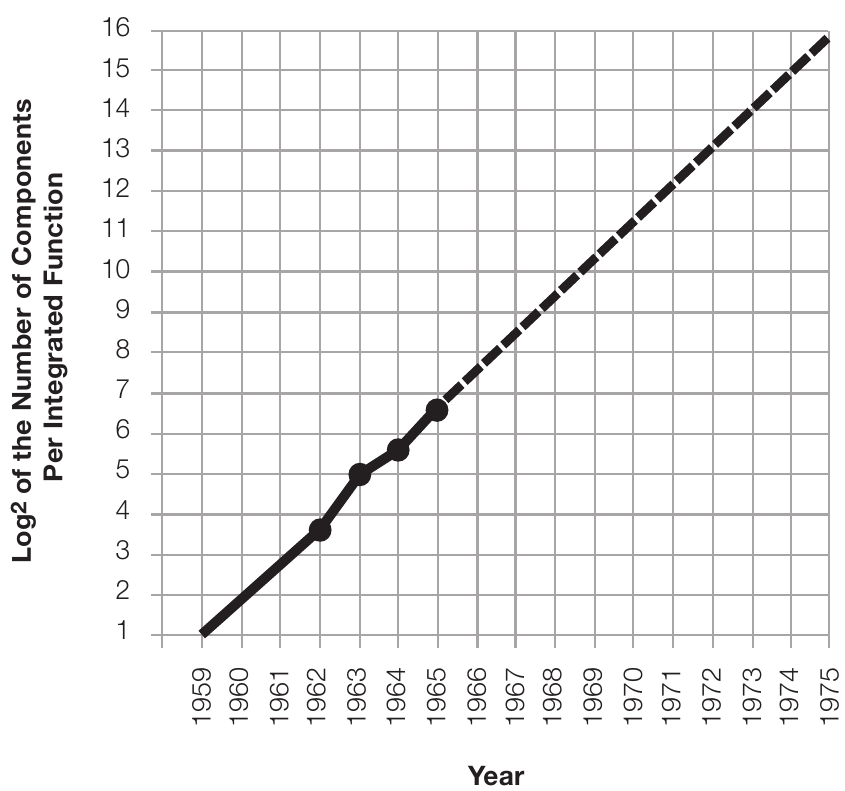
\includegraphics[width=150px]{moore_prediction.png}
\end{figure}


This thesis is centered on program layer\footnote{The program layer 
bring together the program itself, programming models, frameworks and libraries.}. 
This layer is the actual implementation of the algorithm, i.e. where programmers
transforms algorithm to  semantic code that can be transformed lately into
executable binary by compilers. This layer is indeed the interface between pure 
algorithm and the machine architecture. Having an efficient algorithm
mathecamically speaking is not enforcing having an efficient program 
because at algorithm level we do not care about the machine. 
The mechanism to assess the quality in terms of performance are the {\bf performance 
analysis tools} that allows to analyze and detect the bottlenecks. 
There are two main trends, by one hand we have the profilers and by other hand trace
tools. Profiler tools provide performance summaries. This summaries provides 
coarse-grain information, with low-overhead. It means that you can feel the problem 
and infer what could be the origin but the information is not enough if you want 
to be sure. For gather more detail, the other typical approach are the tracing 
tools. High accurate and detailed information can be obtained, but it needs 
more resources in terms of cpu, disk and analyst effort because more data implies 
more complexity. This demand of resources becomes worst since the capacity in 
terms of parallelism is increasing, so the number of tasks to monitor makes 
tracing by one hand hardly scalable and by the other hand tricky to analyze
because the huge quantity of data and because the increasing response times
during the interactive exploration of analysis results. 

Researchers are currently facing this two drawbacks. There are currently several
specialists driving research in the scalability field, they are trying to reduce 
the overhead of tracing in terms of time and trace sizes by mean of several 
techniques like machine learning, data-mining and so on like in 
\cite{llort2015intelligent} or by on-line compression like in
\cite{noeth2009scalatrace}. About analysis field, the complexity of the analysis 
can be overcome by adding intelligence to performance analysis tools, last 
trend is to provide an automatic smart layer that automate an important part 
of the analysis and help the analyzers in their work. Some examples of this 
research line are automatic performance analysis \cite{wolf2003automatic}, 
automatic structure extraction \cite{casas2007automatic}, phases detection 
\cite{gonzalez2013application} fundamental factors models \cite{casas2008aass}, 
automatic analysis throw deep learning \cite{simon:2017:perfdp} and so on.

This thesis is focused on the analysis field and is devoted to humbly contribute 
to ease the work of the analyzers by
automate part of the analysis. The goal of this work is to automatically detect
the internal structure of an application and correlate it with performance metrics by
mean of a post-mortem trace analysis that will help analyzers to have a general
overview about what is actually going on. So instead of deal with whole
information from the very beggining, this approach let the analyzer to figure
out to what part of the gathered information focus on, speeding up the process of
analysis. Also helps to correlate performance analysis with source code, 
since the detected application structure would be similar as
code structure and will contain source coude information that will allow to
easly pinpoint one metric to the code. The structure representation will ignore 
implementation details what therefore will contribute to faster and therefore better 
quality reports for developers. The implementation has been done also thinking 
in techniques of trace size reductions, in particular sampling, so is prepared 
for future developments where the traces do not contain the whole execution behavior.

% TODO
% He visto que todos los trabajos anteriores han intentado resolver el problema
% tirando de una forma o de otra de tecnicas de pattern mining. El coste de este
% tipo de algoritmos es presumiblemente alto, por lo que recuerdo haber leido de
% suele ser cuadrático. De todos modos tengo un survey sobre pattern minning que
% quiero repasar para poder atinar más sobre los costes de los algoritmos
% existentes. Esto es una motivacion desde que el tamaño de las trazas crece
% constantemente y necesitamos algoritmos más eficientes. La tesis que se
% sostiene aquí es que la detección de la estructura interna de las aplicaciones
% puede entenderse como un problema de clasificacion, es decir, clasificar los
% callstacks en conjuntos que vendrian a ser los bucles. El algoritmo por
% excelencia de clasificacion (en base a unas metricas) es el clustering, el
% cual tiene un coste, en el caso del density based clustering de casi-lineal.


\section{Motivation}

High performance computers becomes more complex every generation. The number of 
processors is increasing dramatically, e.g. the current number one on the Top500
 list\footnote{Top500 is the list of the top 500 most powerful high performance 
computers in the world. It is updated two times per year.} is the Sunway TaihuLight 
with 10,649,600 cores\cite{top500_2017} and the trend is even increment this
numbers because the exa-scale era. Analyze application with this quantity 
of processes with fine-grain detail becomes a really tough task when not
impossible because of the huge amount of information. The typical tools like 
visualizers are not enough. One of the major challenges is to
identify and present the hot spot. The researchers demands tools that ease the 
process of performance analysis therefore the main motivation of this work is to ease 
this analysis by means of reducing execution traces to the minimal and meaningful 
expression.

We can say that HPC applications shares a common idiosyncrasy between them. 
Mathematic solvers needs to iterate again and again until the result converge and 
simulation software are used to be programed to evolve over timesteps. So in 
general, HPC applications consists on a big outer loop that is being executed 
again and again the same code but with evolving data, i.e. SPMD\footnote{Single
Program Multiple Data} programs. Additionally this kind of workloads are used
to be burst syncrhonous, i.e. all ranks are executing computation and
communication phases in a syncrhonous manner. For these so regular executions a
relatively simple representation of the whole execution could be extracted, i.e.
the trace could be reduced to a minimum pseudo-code expression
with aggregated data for the whole loop so its somehow folding all the iterations
space. This pseudo-code expresses indeed the actual internal structure of the 
application.

There are previous works (discussed widely on section \ref{related_work})  that 
tries to represent the internal structure of an application but they are used to
use directed graphs like in \cite{aguilar2016event} or just callstack trees like
in \cite{saviankou2015cube}. The drawback of represent the application structure
just with directed graphs is that it is a so simplified view, in the referenced
case it is impossible to pinpoint a given loop (directed graph cycle) to the
actual code because the lack of callstack information. In case of the
referenced approach that uses callstacks tree, the lack of information becomes
from the fact that there is no representation for loops (although you have fuzzy
clues like see the number of calls). In this thesis the proposal is to 
generate a pseudo-code with loop and conditional structures that can be easily 
pinpointed to source code and additionally can show aggregated metrics
that will allow the analyzer to detect the interesting parts to analyze in next
steps. So it can be understood as a sort of mix of the two approaches references
above.

About the used methodology, it can be considered a disruption in this field. The
previous proposals are used to drive this problem using pattern mining
techniques (the basic idea of these algorithms are exposed on section
\ref{pattern_mining}). That is the obvious choice because a trace is basically a
sequence of events sorted by time. The problem with these sort of algorithm are
the cost what are used to be polinomical with a degree of two. {\bf Check
this numbers} Taking into account the exponential increassing of traces sizes 
this thesis mainly contribution is the idea to perform intern 
structure analysis instead of as a pattern mining problem, as a classification
problem. Classification algorithms like clustering presents much better
performance with about quasy-lineal costs.

Summarizing, the main motivation is to speedup the analysis process. In section
\ref{s:pt_evironment} the current analysis flow approach and how it can be
improved by using the tool proposed in this paper is explained.

\section{Sequential pattern mining}\label{pattern_mining}

Traces are basically logs that gather information of the execution of an
application. In a more abstract way, we can define traces just as a sequences
of time ordered events. The fundamentals of recognize the intern structure of an
application is about recognize loops that are those structures in code that
repeats the code into their body as many times as programmer want. Loops in
traces has been unrooled and presents its dynamic aspect. So we can define loops
as a subsequences of instructions that are repeated several times. The work of
identifying loops in traces is about identifying these repetitive subsequences.

Sequential pattern mining can be defined as: \textit{``Given a set of data sequences, the
problem is to discover subsequences that are frequent, that is, the percentage of
data sequences containing them exceeds a user-specified minimum support.''}. Note 
this definition fits pretty well with our objective of loops recognition in traces 
so sequential pattern mining is the natural choice. Furthermore there is another
definition that fits even better for our problem. It is, refering to patterns to
analyze in a temporal sequences:\textit{``\ldots a collection of events that
occur relatively close to each other in a given partial order, and \ldots
frequent episodes as a recurrent combination of events''}.

Sequential pattern mining is a technique applied on a wide range of problems
like for example predicting systems failure by analyzing a sequence of logs,
characterize suspicious behaviour in users by analyzing the sequence of commands
entered, for automatically determine “best practices” by analyzing the sequences
of actions of an expert, etc so the evolution on this area has been quietly
ad-hoc to every problem. On this section pattern mining is introduced and three
main classes of algorithms are explained always from an abstracted point of
view, i.e. without entering into details for specific implementations. This
explanations were taken from \cite{mooney2013sequential}. Even if the temporal
sequences algorithms described in section \ref{ss:temporal_sequences} seems to
be the better choice for structure detection, it has been considered to explain
briefly the other types.

\subsection{Formal notation}

Items are literals that belongs to a given alphabet $I=\{i_{1}, i_{2}, \dots,
i_{m}\}$. Then an event is stated as a non-empty unordered set of items
$(i_{1}, i{2}, \dots, i_{k})$. Finally a sequence is an ordered list of
events $\langle\alpha_{1} \rightarrow \alpha_{2} \rightarrow \dots \rightarrow
\alpha_{q}\rangle$. The ordered metric can be time, space or other. When a
sequence is refered as a $k-sequence$ means that this sequence contains $k$
items. A sequence $\langle\alpha_{1} \rightarrow \alpha_{2} \rightarrow \dots 
\rightarrow \alpha_{n}\rangle$ is a subsequence of $\langle\beta_{1} \rightarrow 
\beta_{2} \rightarrow \dots \rightarrow \beta_{m}\rangle$ if there exists
integers $i_{1}, i_{2}, \dots i_{n}$ s.t. $\alpha_{1} \subseteq \beta_{i_{1}}, 
\alpha_{2} \subseteq \beta_{i_{2}}, \dots, \alpha_{n} \subseteq \beta_{i_{n}}$.
So for example $\langle B \rightarrow AC\rangle$ is a subsequence of 
$\langle AB \rightarrow E \rightarrow ACD \rangle$ being the set of integers 1
and 3.

Having a set of sequences $D$, {\it support} or {\it frequency} of a sequence,
denoted as $\sigma(\alpha, D)$, is defined as the number of input sequences in $D$
that contain $\alpha$. A sequence is {\it frequent} or not depending on a
threshold named {\it minimum support}, so is frequent if it happens more than
{\it minimum support} times. The set of frequent k-sequences is denoted as
$L_{k}$. Moving on, a frequent sequence is {\it maximal} if it is not subsequence
of any other frequent sequence. The task becomes to find all maximal frequent
sequences from $D$.

This definition is a general abstracted definition and can be adapted for
ad-hoc algorithms so for example for the topic we are aware of, items can be the
MPI calls. In this case the
definition of subsequence can be transformed to “if there exists integers 
$i_{1}, i_{2}, \dots i_{n}$ s.t. $\alpha_{1} = \beta_{i_{1}}, 
\alpha_{2} = \beta_{i_{2}}, \dots, \alpha_{n} = \beta_{i_{n}}$” because all
events are sets of one item. If we use the whole callpath instead of just the
MPI call and items are the different calls, now events can not be unordered set
of items but ordered. 

\subsection{Apriori-based algorithms}

Mining frequent itemsets is the core of later analysis like mining association
rules, correlations, sequential patterns and so on. Apriori first proposal was
about discover intra-transaction associations used
in database mining, also called knowledge discovery.
Being $I=\{i_{1}, i_{2}, \dots,i_{m}\}$ a set of literals called items and T a
transaction $T \subseteq I$ is said T contains X if $X \subseteq T$. Further, an
association rule is an implication of the form $X \Rightarrow Y$ where $X
\subset I$, $Y \subset I$ and $X \cap Y = \emptyset$. Apriori algorithm was
presented in the following paper \cite{agrawalfast}. The basis of this algorithm
is presented here and several later algorithms were based on this like for
example AprioriAll, AprioriSome, DynamicSome, GSP (Generalized Sequential
Patterns), PSP and so on. Every one of them are introducing several
optimizations and varying mainly the candidates generation step (explained on
section \ref{ss:discovering_large_itemsets}) but maintains 
the basic core.

The algorithm consists on two fundamental steps being the first the really
challenging one.
\begin{enumerate}
  \item Find all sets of items (itemsets) that have transaction support above
    minimum support.
  \item Use the large itemsets (itemsets above minimum support) to generate the
    desired rules.
\end{enumerate}

\subsubsection{Discovering large itemsets}\label{ss:discovering_large_itemsets}

The large itemsets discovering implies several passes over the data. The first
pass which individual items are actually large, so which of the appears more
than minimum support. On next pass these large items are the seeds, with these
seeds the candidate itemsets are generated and the data is passed again in order 
to find out the large itemsets among the candidates. The same process is repeated 
until no new large itemsets are found. The basic intuition is that any subset of
a large itemset must be large. The algorithm looks like as in pseudocode
\ref{pc:apriori}.

The key point in this algorithm is the candidates generation. It is formed by
two steps. The first step is to generate all the candidates and the second is to
prune those candidates that for sure will not be large itemsets. First step is
represented in pseudocode \ref{pc:apriori_candidate_generator1} and it can be
seen that seed itemsets (from previous pass) are merged in pairs by adding last
item from first itemset to the second. Last phase depited in
\ref{pc:apriori_candidate_generator2} is about prune the candidates
that contain (k-1)-itemsets that do not exists on $L_{k-1}$. The idea behind
that is what has been exposed before, i.e. any subset of a large itemset must
be large. This property leads to a the powerful pruning. By doing that, the 
number of candidates is reduced considerably. By this approach is achieved 
that $C_{k} \supseteq L_{k}$. Ideally $C_{k} = L_{k}$
so as better the prune process is, less verifications (whether the minimum
support is achieved or not) will be done and so better performance.

\begin{pseudocode}{Apriori algorithm}{D}
\label{pc:apriori}
    L_{1} \GETS large \quad 1-itemset
	\\
    \FOR k=2; L_{k} \neq \emptyset; k++ \DO
	\BEGIN
        \COMMENT{New candidates} \\
        C_{k} \GETS aprioriGen(L_{k-1})\\
        \FORALL transactions \quad t \in D \DO
        \BEGIN
            \COMMENT{Candidates contained in t} \\
            C_{t} \GETS subset(C_{k}, t)\\
            \FORALL candidates \quad c \in C_{t} \DO
            \BEGIN
                c.count++\\
            \END\\
        \END\\
        L_{k} \GETS \{c \in C_{k} \mid c.count \geq minsup\}
	\END\\
	\\

    \RETURN \bigcup_{k}L_{k}
\end{pseudocode}

\begin{pseudocode}{Apriori Candidate Generator 1}{L_{k-1}-itemsets}
\label{pc:apriori_candidate_generator1}
\text{ {\bf insert into}} \quad C_{k}\\
\text{ {\bf select}} \quad p.item_{1},\ldots,p.item_{k-1},q.item_{k-1}\\
\text{ {\bf from}} \quad L_{k-1} \quad p,L_{k-1} \quad q\\
\text{ {\bf where}} \quad p.item_{1},\ldots,p.item_{k-2} = q.item_{k-2}, 
p.item_{k-1} < q.item_{k-1}\\
\COMMENT{Last condition is for ensuring no duplicates}
\end{pseudocode}


\begin{pseudocode}{Apriori Candidate Generator 2}{L_{k-1}-itemsets, C_{k}}
\label{pc:apriori_candidate_generator2}
    \FORALL itemsets \quad c \in C_{k} \DO
    \BEGIN
        \FORALL (k-1)-subsets \quad s \in c \DO
        \BEGIN
            \IF s \not\in  L_{k-1} \THEN
                delete \quad c \quad from \quad C_{k}\\
        \END
    \END
\end{pseudocode}

Names used to be so descriptive and therefore can explain quite a lot about the
reality of the entity. Apriori meaning (by oxford dictonary) is {\it “using facts or
principles that are known to be true in order to decide what the probable
effects or results of something will be [\dots]”}. In this case, the name comes
from the generation-and-test technique. A priori, all candidates formed by
(k-1)-itemsets combinations are k-itemsets but it have to be tested.

\subsection{Projection-based pattern growth algorithms}

Candidates generation presents to be critical for apriori algorithms and even if
optimizations in the prune process has been introduced, the generated candidates
follows an exponential grow. For example for detect a maximal sequence of 100
elements, $2^{100} \approx 10^{30}$ candidates will be generated. The next
problem is that for every step, data needs to be revisited to check out whether 
new candidates are large itemsets or not. 

Pattern growth paradigm presented in \cite{han2000mining1} remove
completelly the necesity of candidates generation. They achieve improvements on
performance for about one order of magnitude respect Apriori-like algorithms
explained on previous section by adding two key concepts. 
\begin{enumerate*}[label=(\roman*)]
  \item frequent pattern tree or FP-tree for short
  \item and FP-tree based pattern mining called FP-growth.
\end{enumerate*}
Following this two concepts are explained in more detail.

\subsubsection{Frequent pattern tree}

The following observations can be used for introduce FP-trees and have been used
for its construction. This structure dramatically decrease the size of data to be 
scanned but maintains all the need information for the mining.

\begin{enumerate}[label=\roman*)]
  \item One important rule learned from apriori approach is that frequent
    k+1-itemsets only can be done from frequent k-itemsets. This observacion
    leads to the idea of just taking into account frequent 1-itemsets given a
    minimum support.
  \item These discovered frequent intemsets could be stored in some compact
    structure, avoiding repeatedly scanning the DB.
  \item Continuing with the idea of compacting importante data, it can be said
    that identical frequent itemsets from different transactions can be merged
    into one with information about number of occurrences.
  \item And for these partially identical frequent itemsets, shared prefixes can
    be merged as well.
\end{enumerate}

For improve understandability lets drive a construction of an FP-tree following an
example. Imagine we have a database with several transactions like the depicted
in figure \ref{fig:fp_tree_db} (left hand side column). The process ends up with
Fp-tree in figure \ref{fig:fp_tree_constructed}. Lets see how it happens. 

First scan of database derives a list of frequent items, i.e. these 1-itemsets 
above the minimum support value (3 for this example) that is $\langle
(f:4),(c:4),(a:3),(b:3),(m:3),(p:3) \rangle$. Note the frequent items in every
transaction are on right hand side column in figure \ref{fig:fp_tree_db}. The
frequent itemsets here are not sorted by appearance in transaction but by
frequence. This sorting will allows more compression on FP-tree construction.

The second scan is done over these frequent 1-itemsets and drives the
FP-tree construction. First transaction leads to the construction of the first
branch (left hand side). Next transaction shares the three first items, so
it can be partially merged with first branch. The merge process is just about
update the counters and make the new relations. Same process for all
transactions.

\begin{figure}
  \centering
  \includegraphics[width=250px]{fp_tree_db}
  \caption{A transaction database as running example}
  \label{fig:fp_tree_db}
\end{figure}

\begin{figure}
  \centering
  \includegraphics[width=200px]{fp_tree_constructed}
  \caption{The FP-tree}
  \label{fig:fp_tree_constructed}
\end{figure}

Additionally to the pure tree construction, header table structure is done for
ease the task of traverse all possible frequent patterns that contains a given
item. 

\subsubsection{Mining FP-trees}

After prepare data, FP-growth algorithm is the responsible to find out the
frequent patterns by analyzing the FP-tree. The mining starts with 1-itemset
analysis. Thanks to the header table all paths for a given item $a_{i}$ can be get
easily. Once all paths where the given item is involved on are retrieved a new 
subtree is build up. Remember that in this process all items below minimum support 
are pruned. Unlike before now only these retrieved items are taken into account 
for the counting. This new structure is named $a_{i}$ conditional pattern base,
i.e. the sub-pattern base under the condition of $a_{i}$ existence. Next step is
to call mining function recursively having on every recursive call a large
conditional pattern base, so it is growing. It can be better understood by means
of an example. Lets follow the previous one.

Starting from the bottom of the header table, lets mine FP-tree fora $p$ item. Two
paths arise: $\langle f:4,c:3,a:3,m:2,p:2 \rangle$ and $\langle c:1, b:1, p:1
\rangle$ (being the number after ``:'' the occurrences). Note that even if $f$
appears 4 times, only 2 of them appears with $p$, so the path becomes $\langle 
f:2,c:2,a:2,m:2,p:2 \rangle$. Similarly with second path. Moving on, the
construction of the $p$ conditional pattern base is done by counting and pruning
these items below minumum support, so the only branch for the new FP-tree is
$(c:3)$. Hence only one frequent pattern is derived, i.e. $(cp:3)$. From now to
the end, $p$ does not need to be taken into account any more, this is because
all possible patterns containing $p$ has been already analyzed. Similarly we can proceed analyzing paths containing $m$ item. Two paths arise: 
$\langle f:2,c:2,a:2,m:2 \rangle$ and $\langle f:1,c:1,a:1,b:1,m:1 \rangle$. The
new conditional FP-tree just contains the path $\langle f:3,c:3,a:3 \rangle$.
For show how the pattern is growing, lets see in a deph-first way what
recursive calls are done:
\begin{enumerate*}[label=(\roman*)]
  \item mine($\langle f:3,c:3,a:3 \rangle \text{\textbar} m$)
  \item mine($\langle f:3,c:3 \rangle \text{\textbar} am$)
  \item mine($\langle f:3 \rangle \text{\textbar} cam$)
\end{enumerate*}
The frequent pattern derived from this analysis is $(fcam:3)$.

\subsection{Temporal sequences}\label{ss:temporal_sequences}

In this section will be shown the basis of these algorithms that concers about
the periodicity of a certain patterns over the time. These are obviusly the
algorithms that best fits to the needs for trace structure detection. First
developed framework for datasets considered to be episodic was presented by
\cite{mannila1995discovering}.

Two previous approaches were concerning about the analysis of arbirary ordered
sequences of data, however, this approach considers order as an inherent
characteristic of the sequential structure. This main difference leads to a
different approach of sequential pattern mining and introduce new ideas like
sliding windows. Nevertheless some important components are shared among them like:
\begin{enumerate*}[label=(\roman*)]
  \item Frequency threshold, that is defined as the minimum number of times a
    sequence have to appear. It is analogous to minimum support of apriori and
    pattern-growth algorihtms.
  \item Relies on generate-and-test paradigm to discover frequent sequences. It
    is same approach like apriori-like algorithms.
  \item Finnaly also takes profit from the principle of: all subepisodes are at
    least as frequent as the superepisode, for candidates generation.
\end{enumerate*}

\subsection{Use in structure detection and discussion}

Seems that projection-based patter growth algorithm is what is most used in
semantic structure detection. Reference to state of the art for that. Discuss
how both types of algorithms can be used for this purpose and also and more
important discuss the complexity of those algorithms. Maybe just an introduction
of a real discussion because it should be done on methodology chapter.


\section{Clustering techniques}

Hola manola


